%% ==============================
\chapter{Single-bidder and Single-item Randomization Auction}
\label{ch:body of thesis}
%% ==============================
In this chapter, we evaluate APX with different probability distribution under single-bidder and single-item randomization auction experiment. We still use \textit{take-it-or-leave-it} auction mechanism. The robust paper defines a specific \textit{randomized} selling mechanism, which essentially corresponds to the lottery proposed by Carrasco et al. [paper reference]
\begin{definition}[Log-Lottery]
	\label{definition:loglottery}
	Fix any $\mu > 0$ and $\sigma \geqslant 0$. A log-lottery is a randomized mechanism that sells at a price $P^{log}_{\mu,\sigma}$, which is distributed over the nonnegative interval support $[\pi_1, \pi_2]$ according to the cdf
	\begin{equation}\notag
		F^{log}_{\mu,\sigma} (x) =  \frac{\pi_2 \ln\frac{x}{\pi_1} -(x - \pi_1)}{\pi_2 \text{ln} \frac{\pi_2}{\pi_1} - (\pi_2-\pi_1)}
	\end{equation}
	where parameters $\pi_1,\pi_2$ are the (unique) solutions of the system
	\begin{equation}
		\begin{cases} \pi_1 (1 + \text{ln}\frac{\pi_2}{\pi_1}) = \mu   \\    \pi_1(2\pi_2 - \pi_1) = \mu^2 + \sigma^2  \end{cases}
	\end{equation}
\end{definition}
We will sometimes slightly abuse notation and use $P^{log}_{\mu,\sigma}$ to refer both the log-lottery mechanism and the corresponding variable of the prices.

This time, we sample $N$ $P^{log}_{\mu,\sigma}$s from log-lottery distribution (i.e. $N = 10000$), and for each $P^{log}_{\mu,\sigma}$ we perform our Auction Experiment Procedure \ref{alg:auctionexperiment} from Chapter 2. We just need replace $p_D$ with $P^{log}_{\mu,\sigma}$ in the procedure. 
\section{Log-Lottery Randomization}
The log-lottery distribution defined in Definition \ref{definition:loglottery} is not a regular distribution, therefore there is no sampling function in Python we can use directly. For this distribution we can use rejection a sampling technique. First we need to check its pdf
\begin{equation}\notag
	f^{log}_{\mu,\sigma} (x) =  \frac{\pi_2\frac{1}{x} -1}{\pi_2 \text{ln} \frac{\pi_2}{\pi_1} - (\pi_2-\pi_1)}
\end{equation} \label{eq: llequation}
$f^{log}_{\mu,\sigma} (x)$ is monotone decreasing on $[\pi_1,\pi_2]$, so $\text{max}(f^{log}_{\mu,\sigma} (x)) = f^{log}_{\mu,\sigma} (\pi_1)$.
Since this distribution is bounded on bounded support, we can indeed use a rejection sampling technique by proposing an uniform density
\begin{center}
	$q(x) = \begin{cases} \frac{1}{\pi_2 - \pi_1}  & \text{if } x \in [\pi_1, \pi_2] \\ 0   & \text{otherwise } \end{cases}$
\end{center}
A constant $A = f^{log}_{\mu,\sigma} (\pi_1)\cdot (\pi_2 - \pi_1)$, then we know $A \cdot q(x) \geqslant	f^{log}_{\mu,\sigma} (x) , 	\forall x \in [\pi_1,\pi_2]$. Our rejection sampling steps can be described in Algorithm \ref{alg:boundRejection} below.
\begin{algorithm}[H]
	\caption{Rejection Sampling Algorithm}\label{alg:boundRejection}
	\begin{algorithmic}[1]
		\Procedure{Rejection Sampling}{N}
		\State $n \gets 0$
		\State $x_{list}$ is empty
		\While{$n  \leqslant N$}\Comment{N is sample size}
			\State draw $x \sim q(x)$		
			\State compute acception probability $a := \frac{f^{log}_{\mu,\sigma} (x) }{Aq(x)}$
			\State draw a random sample $u \sim U[0,1]$
			\If{$u \leqslant a$}
				\State accept $x$, add it to $x_{list}$
				\State $n\gets n+1$	
			\EndIf
		\EndWhile
		\State \textbf{return} $x_{list}$
		\EndProcedure
	\end{algorithmic}
\end{algorithm}
For example, if we have a $\mu = 1$ and $\sigma = 1$ log-lottery distribution, we can solve $\pi_1, \pi_2$ using system of equation \cref{eq: llequation}. We get $\pi_1 = 0.2778$ and $\pi_2 = 3.7383$ from the numerical solver. Histogram in \cref{fig:rejectionS} shows the density of samples from our rejection sampling algorithm and the green line represents the corresponding pdf of the log-lottery distribution.
\begin{figure}[H]
	\centering
	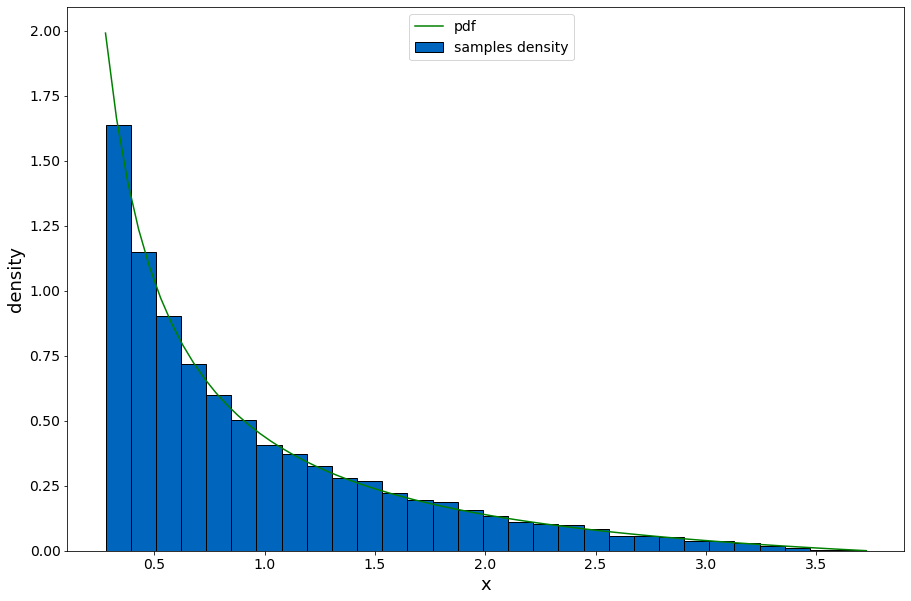
\includegraphics[width=1\textwidth]{rejectionS}
	\caption{The actual log-lottery pdf and the results from rejection sampling algorithm}
	\label{fig:rejectionS}
\end{figure} 

In our new randomised auction experiment, we keep exact same steps from Auction Experiment \ref{alg:auctionexperiment} to simulate the OPT$(F)$. The only difference is simulating the expected revenue REV$(F)$, since now our $p_D$ is not a fixed value but a random number from a log-lottery distribution. Thus in order to simulate the expected revenue, we first draw $x_{list}$ (contains $N$ random samples) using above \cref{alg:boundRejection}, and for each reserve price in $x_{list}$ we simulate $n$ auction experiments. Then we will have $N$ revenue outputs from the auction experiments, and we take the average of these $N$ values and this average is our final expected revenue $\text{REV}(F)$.


\newpage
\section{Different Valuation Distributions}
In this section, we want to see how the expected revenue and APX will be under different valuation distributions.
\subsection{Uniform distribution}
If our bidder's valuation is from a uniform distribution, this time our reserve price is randomly draw from $P^{log}_{\mu,\sigma}$ while other parameters remain the same, given $U[a,b]$, under the log-lottery randomization selling mechanism, we can write down our expected revenue with reserve price $P^{log}_{\mu,\sigma}$  
\begin{equation}\notag
\begin{split}	
	\text{REV}(P^{log}_{\mu,\sigma} ;U[a,b]) &=\underset{ p \sim F^{log}_{\mu,\sigma} }{\mathbb{E}}\left[ p(1-F_{uniform}(p))\right] \\ &= \int_{\pi_1}^{\pi_2} p(1 -  \frac{p-a}{b-a})f^{log}_{\mu,\sigma}(p)dp\\ &=\int_{\pi_1}^{\pi_2} p(1 -  \frac{p-a}{b-a}) \cdot \frac{\pi_2\frac{1}{p} -1}{\pi_2 \text{ln}\frac{\pi_2}{\pi_1} - (\pi_2-\pi_1)} dp \\&=\int_{\pi_1}^{\pi_2} \frac{p(b-p)}{b-a} \cdot \frac{\pi_2 -p}{p(\pi_2 \text{ln}\frac{\pi_2}{\pi_1} - (\pi_2-\pi_1))} dp \\&=  \frac{1}{(b-a)(\pi_2 \text{ln}\frac{\pi_2}{\pi_1} - (\pi_2-\pi_1))}\int_{\pi_1}^{\pi_2} (b-p)(\pi_2-p)dp\\&=  \frac{1}{(b-a)\left(\pi_2 \text{ln}\frac{\pi_2}{\pi_1} - (\pi_2-\pi_1)\right)} \cdot \left( \frac{p^3}{3} -\frac{bp^2}{2} -\frac{\pi_2p^2}{2} + b\pi_2 p \Biggr|_{\pi_2}^{\pi_1} \right)              
\end{split}
\end{equation} 

From Chapter 2, we also know $\text{OPT}(U[a,b]) = \frac{b^{2}}{4(b-a)}$, then
\begin{equation}\notag
    \text{APX} = \frac{\text{OPT}(U[a,b])}{\text{REV}(P^{log}_{\mu,\sigma} ;U[a,b])} = \frac{b^2\left(\pi_2 \text{ln}\frac{\pi_2}{\pi_1} - (\pi_2-\pi_1)\right)}{4\left( \frac{p^3}{3} -\frac{bp^2}{2} -\frac{\pi_2p^2}{2} + b\pi_2 p \Biggr|_{\pi_2}^{\pi_1} \right)  }
\end{equation}
As we can see, the expected revenue expression under randomization gets more complex comparing to the deterministic one. We will use our experiment simulation to determine APX experimentally, and results are presented in next section. 

\subsection{Truncated Normal Distribution}
Similarly the expected revenue of a truncated normal distribution TN$(\hat{\mu}, \hat{\sigma}^2, 0, \infty)$

\begin{equation}\notag
\begin{split}	
	\text{REV}(P^{log}_{\mu,\sigma} ;\text{TN}(\hat{\mu}, \hat{\sigma}^2, 0, \infty)) &=\underset{p \sim F^{log}_{\mu,\sigma} }{\mathbb{E}}\left[ p(1-F_{\text{TN}}(p))\right] \\ &= \int_{\pi_1}^{\pi_2} p(1 -  F_{\text{TN}}(p))f^{log}_{\mu,\sigma}(p)dp \\&=\int_{\pi_1}^{\pi_2} p(1 - F_{\text{TN}}(p) )\cdot \frac{\pi_2 -p}{p(\pi_2 \text{ln}\frac{\pi_2}{\pi_1} - (\pi_2-\pi_1))} dp \\&=  \frac{1}{\pi_2 \text{ln}\frac{\pi_2}{\pi_1} - (\pi_2-\pi_1)}\int_{\pi_1}^{\pi_2} (1 -  F_{\text{TN}}(p))(\pi_2-p)dp 
\end{split}
\end{equation} 
where $F_{\text{TN}} = \frac{\Phi(\frac{x- \hat{\mu}}{\hat{\sigma}}) - \Phi(\frac{- \hat{\mu}}{\hat{\sigma}})}{1 - \Phi(\frac{- \hat{\mu}}{\hat{\sigma}})}$.\\
For truncated normal distribution, there is a nonlinear integration term in its expected revenue expression, which is even more complex. Thus we will not explore further on the expression of APX in this case. 
\subsection{Pareto Distribution}
We first consider $\text{Pareto}(1)$ distribution, whose support is $[1, \infty)$. 
\begin{equation}\notag
\begin{split}	
	\text{REV}(P^{log}_{\mu,\sigma} ;\text{Pareto}(1)) &=\underset{p \sim F^{log}_{\mu,\sigma} }{\mathbb{E}}\left[ p\left(1-F(p)\right)\right] \\ &= \int_{\pi_1}^{\pi_2} p\left(1 -  (1-\frac{1}{p^c})\right)f^{log}_{\mu,\sigma}(p)dp \\&=\int_{\pi_1}^{\pi_2} p^{1-c}\cdot \frac{\pi_2 -p}{p(\pi_2 \text{ln}\frac{\pi_2}{\pi_1} - (\pi_2-\pi_1))} dp \\&=  \frac{1}{\pi_2 \text{ln}\frac{\pi_2}{\pi_1} - (\pi_2-\pi_1)}\int_{\pi_1}^{\pi_2} p^{-c}(\pi_2-p)dp 
\end{split}
\end{equation} 
We know the OPT$\left(\text{Pareto}(1)\right) = 1$, then
\begin{equation}\notag
    \text{APX} = \frac{\text{OPT}\left(\text{Pareto}(1)\right)}{\text{REV}(P^{log}_{\mu,\sigma} ;\text{Pareto}
    (1))} = \frac{\pi_2 \text{ln}\frac{\pi_2}{\pi_1} - (\pi_2-\pi_1)}{ \int_{\pi_1}^{\pi_2} p^{-c}(\pi_2-p)dp }
\end{equation}

We can also write down the expected revenue and APX for $\text{Pareto}(0)$ distribution.
\begin{equation}\notag
\begin{split}	
	\text{REV}(P^{log}_{\mu,\sigma} ;\text{Pareto}(0)) &=\underset{p \sim F^{log}_{\mu,\sigma} }{\mathbb{E}}\left[ p\left(1-F(p)\right)\right] \\ &= \int_{\pi_1}^{\pi_2} p\left(1 -  (1-\frac{1}{(p+1)^c})\right)f^{log}_{\mu,\sigma}(p)dp \\&=\int_{\pi_1}^{\pi_2} \frac{p}{(p+1)^c}\cdot \frac{\pi_2 -p}{p(\pi_2 \text{ln}\frac{\pi_2}{\pi_1} - (\pi_2-\pi_1))} dp \\&=  \frac{1}{\pi_2 \text{ln}\frac{\pi_2}{\pi_1} - (\pi_2-\pi_1)}\int_{\pi_1}^{\pi_2} \frac{\pi_2 - p}{(p+1)^c}dp 
\end{split}
\end{equation} 
We know the OPT($\text{Pareto}(0)$) = $\frac{(c-1)^{c-1}}{c^c}$, then
\begin{equation}\notag
    \text{APX} = \frac{\text{OPT}(\text{Pareto}(0))}{\text{REV}(P^{log}_{\mu,\sigma} ;\text{Pareto}(0))} = \frac{\frac{(c-1)^{c-1}}{c^c}\cdot \left(\pi_2 \text{ln}\frac{\pi_2}{\pi_1} - (\pi_2-\pi_1)\right)}{ \int_{\pi_1}^{\pi_2} \frac{\pi_2 - p}{(p+1)^c}dp  }
\end{equation}

It is clear that the expression of expected revenue and APX are getting more complex under randomisation situation. Thus using our experiment simulation becomes more convenient and delicate here to compute the experimental APX. 

\section{Observation and Results}
We present four figures which are the results from different valuation distributions. In each figure, we plot the $r$ with the corresponding APX against the corresponding DAPX. As we can see, for these four distributions: uniform, truncated normal, Pareto(1) and Pareto(2), the experimental DAPX is better/smaller than APX. The robust paper proposed both deterministic selling mechanism and log-lottery randomised selling mechanism, and our experiment shows that for single-bidder and single-item auction the proposed deterministic mechanism performs better than the proposed randomization mechanism. The possible reason to this result will be: for single-bidder and single-item auction, a good deterministic mechanism can perform better than a specific randomised mechanism, in our case, that means log-lottery randomization is probably not a good randomization choice comparing to the proposed deterministic mechanism. 

\begin{figure}[H]
	\centering
	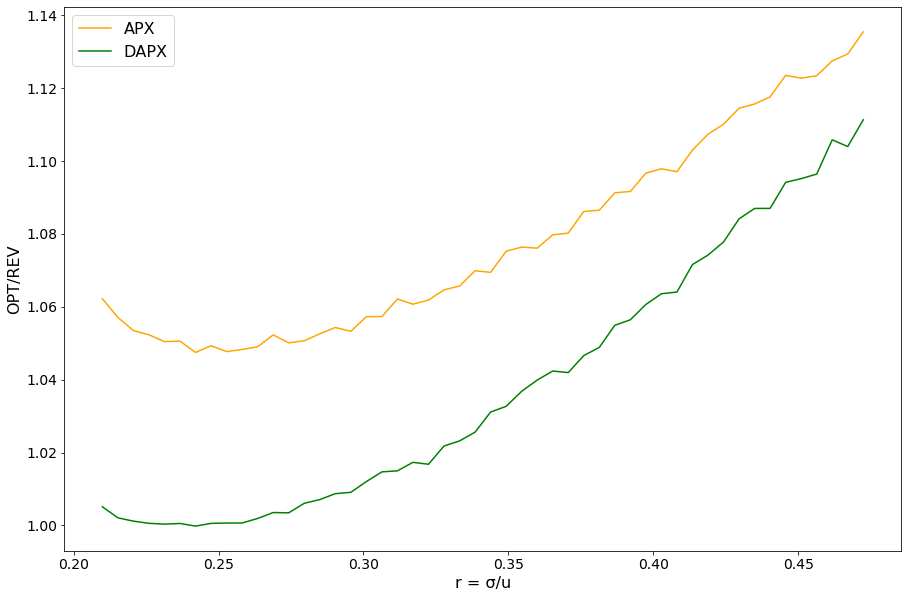
\includegraphics[width=1\textwidth, height=8.5cm]{apxuni.png}
	\caption{Uniform distribution: experimental APX versus DAPX}
	\label{fig:apxuni}
\end{figure}
\begin{figure}[H]
	\centering
	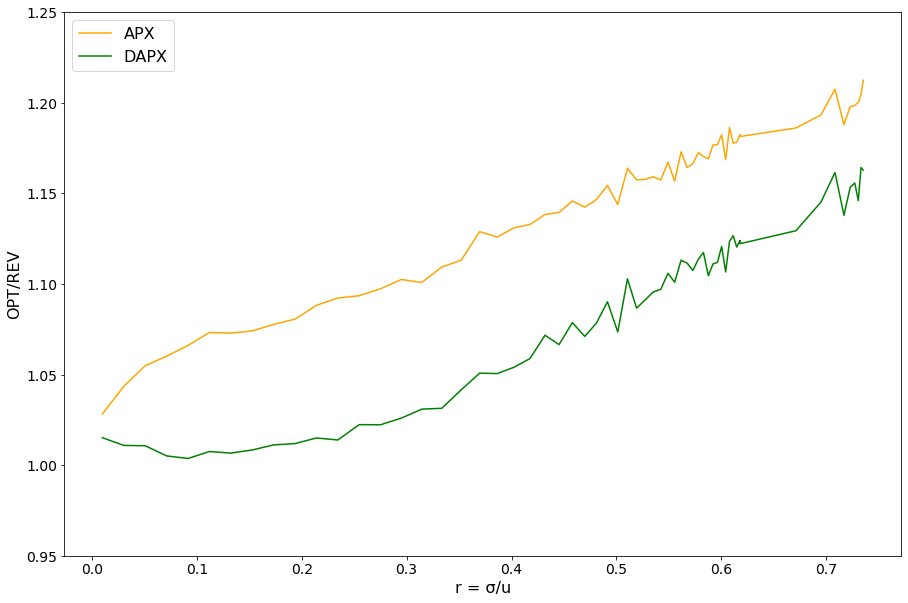
\includegraphics[width=1\textwidth,height=8.5cm]{apxtnorm.png}
	\caption{Truncated normal distribution: experimental APX versus DAPX}
	\label{fig:apxtnorm}
\end{figure}
\begin{figure}[H]
	\centering
	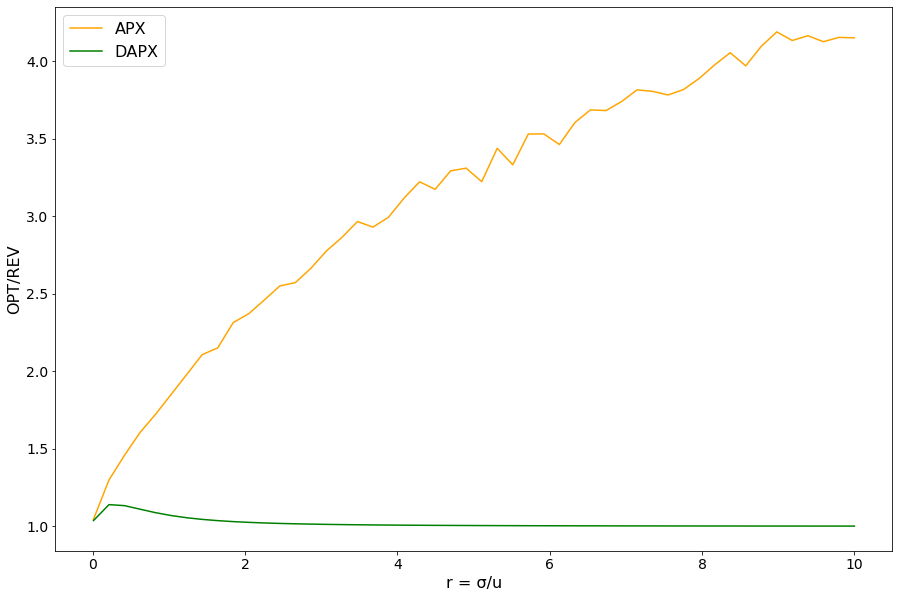
\includegraphics[width=1\textwidth,height=8.5cm]{apxpareto.png}
	\caption{Pareto(1) distribution: experimental APX versus DAPX}
	\label{fig:apxpareto}
\end{figure}
\begin{figure}[H]
	\centering
	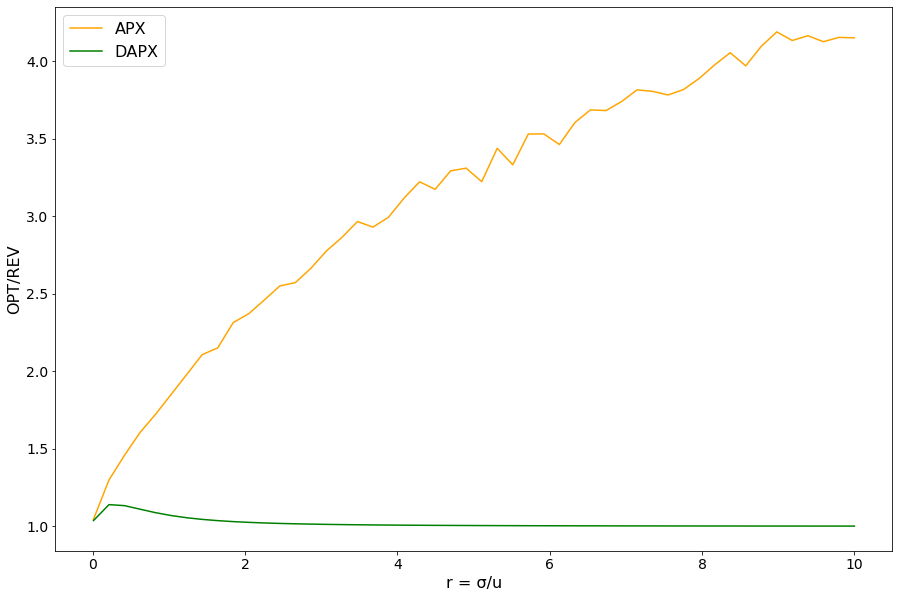
\includegraphics[width=1\textwidth,height=8.5cm]{apxpareto0.png}
	\caption{Pareto(0) distribution: experimental APX versus DAPX}
	\label{fig:apxpareto0}
\end{figure}





However here also comes our questions: in general, randomization is better than deterministic mechanism. Here we compared one deterministic mechanism with one randomization mechanism given a certain valuation distribution. In the paper, APX is the ratio under worst case (worst probability distribution) with log lottery randomization. 

1.Randomization is better than deterministic, but given a valuation distribution, using one specific randomization may not be better. Thus whether log lottery is the best randomization distribution. How about using uniform or truncated normal distribution for price randomization? Especially is log lottery is the best for uniform and truncated normal distribution?
2.During the experiment, we use rejection sampling to generate random log lottery price, is the sample size sufficient enough?
3.A better deterministic mechanism can result a better approximate robust ratio than a specific randomization mechanism, i.e. better than log lottery randomization. However in worse case, APX is always better than DAPX. 






\chapter{Multiple Items}
In this chapter, we consider a single additive buyer with valuations for $m$ items. We start with a simple setting by assuming these $m$ items are independently identical distributed items. First challenge for us is to determine the optimal revenue, the robust paper simply use the welfare bound in the proof for APX upper bound. First one, we are interested in $\text{OPT}(F)$, we propose two feasible deterministic mechanisms to evaluate the lower bound of $\text{OPT}(F)$ in section \cref{sec:multiOR}

\section{Optimal Revenue} \label{sec:multiOR}
In paper...., the optimal revenue is proved up to 5 uniform i.i.d items. Thus even when the items are i.i.d distributed, it is difficult to determine the optimal revenue. We know the upper bound of the optimal revenue is the optimum welfare, $\text{OPT}(F) \leqslant \text{VAL}(F)$. Now we propose two possible "optimal" auction mechanisms for a single additive bidder with $m$ i.i.d items, and we run our experiment according to these two auction mechanisms with different probability distribution. Then we will get two lower bounds for the optimal revenue.\\
Let us denote $A1$ is the mechanism by selling $m$ items separately, i.e. perform $m$ Myerson optimal auctions. Since the bidder's valuation for the items are i.i.d distributed, we have $\text{REV}(A1, F) = \sum^m_{j=1} \text{REV}(p_{opt}, F) = m\text{REV}(p_{opt}, F)$, thus we only need to run our auction experiment algorithm once with the optimal reserve price for the given probability distribution, which we have already done in Section 2. Multiplying the experimental expected revenue with $m$ we get the expected revenue for $A1$ mechanism. Following table shows different distributions we want to test and the optimal reserve price we will use in the experiment and the corresponding expression of $\text{REV}(F)$. The next table shows the tested specific distributions and the corresponding $p_{opt}$ and the experimental values for $\text{OPT}(F)$
\begin{center}
	\begin{table}[H]
		\begin{tabular}{ | m{5cm} | m{4cm} |m{4cm}|  } 
		\hline
		\textbf{Distribution}	&	\textbf{optimal reserve price $p_{opt}$}  & 	\textbf{$\text{REV}(F)$ for m items}   \\ 
		\hline
		Uniform distribution & $\text{max} \{a, \frac{b}{2} \}$ & $m \cdot p_{opt} (1-\frac {p_{opt}-a}{b-a})$  \\ 
		\hline
		Truncated normal distribution & $ \psi_{TN}^{-1}(0)$ & $ m \cdot p_{opt} (1-F_{TN}(F))$ \\ 
		\hline
		 Pareto distribution  ($x \in \left[1,\infty \right)$)& 1 & $m$ \\
		\hline
		 Pareto distribution  ($x \in \left[0,\infty \right)$)& $\frac{1}{c-1}$ & $m \cdot \frac{(c-1)^{c-1}}{c^c}$ \\
		\hline
		\end{tabular}
		\caption{A1: Optimal revenue expression}
		\label{tab:optrevenueEx}
	\end{table}
\end{center}
\begin{center}
	\begin{table}[H]
		\begin{tabular}{ | m{5cm} | m{4cm} |m{4cm}|  } 
		\hline
		\textbf{Distribution}	&	\textbf{optimal reserve price $p_{opt}$}  & 	\textbf{Experimental $\text{REV}(F)$ for 1 item}   \\ 
		\hline
		Uniform distribution & $\text{max} \{a, \frac{b}{2} \}$ & $m \cdot p_{opt} (1-\frac {p_{opt}-a}{b-a})$  \\ 
		\hline
		Truncated normal distribution & $ \psi_{TN}^{-1}(0)$ & $ m \cdot p_{opt} (1-F_{TN}(F))$ \\ 
		\hline
		 Pareto distribution  ($x \in \left[1,\infty \right)$)& 1 & $m$ \\
		\hline
		 Pareto distribution  ($x \in \left[0,\infty \right)$)& $\frac{1}{c-1}$ & $m \cdot \frac{(c-1)^{c-1}}{c^c}$ \\
		\hline
		\end{tabular}
		\caption{A1: Experimental Optimal revenue results}
		\label{tab:optrevenueRE}
	\end{table}
\end{center}
Let us denote $A2$ is the mechanism by selling $m$ items all together, i.e. perform one Myerson optimal auction. To compute the expected revenue for $A2$ we can run our auction experiment algorithm and within the algorithm we generate $m$ random numbers parallel from the probability distribution $F$ and treat the sum of these $m$ random numbers as one bid.

\section{DAPX and APX} 
therefore we can try to evaluate the upper bound of APX. Let's denote our auction mechanism is $A$, and valuation distribution $F$ (i.e. a unifrom distribution) with mean $\mu$ and standard deviation $\sigma$, then the robust approximation ratio of selling m independently ($\mu, \sigma$) - distributed items is:
\begin{equation}\notag
    \text{APX}(\vec{\mu},\vec{\sigma}) = \frac{\text{OPT}(F)}{\text{REV}(A;F)} \leqslant \frac{m\mu}{\text{REV}(A;F)}
\end{equation}
From the Robust paper, it proposes two feasible randomization auction mechanisms, which are:
\begin{itemize}
    \item $A1$ is the mechanism that sells independently each i.i.d item using log-lottery 
    \begin{equation}\notag
        \text{APX}(\vec{\mu},\vec{\sigma}) = \frac{\text{OPT}(F)}{\text{REV}(A1;F)} \leqslant \frac{m\mu}{m\text{REV}(P^{log}_{\mu,\sigma};F)} = \frac{\mu}{\text{REV}(P^{log}_{\mu,\sigma};F)}
\end{equation}
    \item $A2$ is the mechanism that sells all $m$ items together, i.e. price their sum of valuations $Y$ and  using log-lottery 
    \begin{equation}\notag
        \text{APX}(\vec{\mu},\vec{\sigma}) = \frac{\text{OPT}(F)}{\text{REV}(A2;F_Y)} \leqslant \frac{m\mu}{\text{REV}(P^{log}_{\Bar{\mu},\Bar{\sigma}};F_Y)}
\end{equation}
\end{itemize}
Robust paper does not mention it explicitly, but we can also consider another two feasible deterministic auction mechanisms
\begin{itemize}
    \item $A3$ is the mechanism that sells independently each i.i.d item using a fixed reserve price $p_D$, where $p_D = \frac{\rho_D(r)}{2\rho_D(r) - 1} \cdot \mu$, and $r = \frac{\sigma}{\mu}$
    \begin{equation}\notag
        \text{DAPX}(\vec{\mu},\vec{\sigma}) = \frac{\text{OPT}(F)}{\text{REV}(A3;F)} \leqslant \frac{m\mu}{m\text{REV}(p_D;F)} = \frac{\mu}{\text{REV}(p_D;F)}
\end{equation}
    \item $A4$ is the mechanism that sells all $m$ items together using a fixed reserve price $\Bar{p}_D$, where $\Bar{p}_D = \frac{\rho_D(\Bar{r})}{2\rho_D(\Bar{r}) - 1} \cdot \Bar{\mu}$, and $\Bar{r} = \frac{\Bar{\sigma}}{\Bar{\mu}}$, i.e. price their sum of valuations $Y$ and 
    \begin{equation}\notag
        \text{DAPX}(\vec{\mu},\vec{\sigma}) = \frac{\text{OPT}(F)}{\text{REV}(A4;F_Y)} \leqslant \frac{m\mu}{\text{REV}(\Bar{p}_D;F_Y)}
\end{equation}
\end{itemize}

\chapter{Additional notes}
\section{truncated normal distribution part}

\begin{center}
	$f_t(x) = \begin{cases} k f(x) & \text{if } x \geqslant 0 \\ 0   & \text{otherwise } \end{cases}$
\end{center}

where $k$ is a normalizing constant. We can determine k by using the knowledge of the sum of the probablity equals to 1. Then we have: 

\begin{center}
	
	$1 = \int_{R}f_t(x) dx = \int_{0}^{\infty} k f(x)dx = k \cdot \int_{0}^{\infty} f(x) dx$
	
\end{center}

\begin{center}
	
	$\implies k = \frac{1}{\int_{0}^{\infty}f(x) dx } = \frac{1}{1 - F(0)}$
	
\end{center}

Here $x \geqslant 0 $, then the coresponding cdf is:
\begin{center}
	$F_t(x) = \int_{0}^{x} kf(t) dt =  k \cdot \int_{0}^{x} f(t) dt = k(F(x) - F(0))$
\end{center}






question to answer:\\
1.two random variables, X,Y, let Y = c*X where c>0 constant. let $F_X,f_X$ be the cdf, pdf of X what is the relation of $F_Y,f_y$ to $F_X,f_X$\\
$F_Y (y) = P(Y \geqslant y) = P(cX \leqslant y) = P(X \leqslant \frac{y}{c}) = F_X (\frac{y}{c})$\\
we know $f_Y(y) = f_X (g^{-1}(y))|\frac{d g^{-1}(y)}{dy}|$ thus:\\
$f_Y (y) = f_X(\frac{y}{c})\cdot|\frac{1}{c}| =\frac{1}{c}f_X(\frac{y}{c})$\\
2. what is the relation of myerson(Y) and myerson(X)\\
Myerson(X) optimal revenue can be achieved by a deterministic mechanism, let denot $v_x$ of optimal reverse price for X, then OPT(X) = $v_x(1-F_X(v_x))$, what if optimal reserve price for Y?
we can compute optimla reserve price by setting virtual valuation for Y equal to 0:
\begin{align}\notag
v - \frac{1-F_X (\frac{v}{c})}{\frac{1}{c}f_X(\frac{v}{c}) } &= 0 \\     
\notag  \frac{v}{c} - \frac{1-F_X (\frac{v}{c})}{ f_X(\frac{v}{c}) }  &= 0
\end{align}
set $v^{'} = \frac{v}{c}$, above equation has solution $v_x$.
Then denote optimal reserve price for Y: $v_y =c v_x$ then OPT(Y) = $v_y(1 - F_Y(v_y)) =cv_x(1 - F_X(\frac{cv_x}{c})) = cv_x(1 - F_X(v_x))$. Therefore OPT(Y) = cOPT(X)
3. what is the relation of REV(Y) and REV(x), given v as reserve price\\
REV(Y) = $v(1-F_Y(v)) = v(1-F_X(\frac{v}{c}))$\\
REV(X) =  $v(1-F_X(v))$ 
\begin{equation}\notag
\begin{split}	
v(1-F_X(\frac{v}{c})) &\overset{0 < c < 1}{ < }v(1-F_X(v))\\&\overset{c= 1}{ = } \\&\overset{c > 1}{ > }
\end{split}
\end{equation} 




Experiment Evaluation of Robust Revenue-Maximizing Auctions\\ \\


%%% Local Variables: 
%%% mode: latex
%%% TeX-master: "thesis"
%%% End: 